\section{ADDITIONAL EXPERIMENTS}\label{sec:add_expes}

\subsection{\pkg{glmnet} versus \pkg{SLOPE} Comparison}
\label{sec:slope-vs-glmnet}

In this experiment, we ran the \pkg{glmnet}~\parencite{friedman2022} and \pkg{SLOPE}~\parencite{larsson2022d} packages on the \dataset{bcTCGA} dataset, selecting the regularization sequence \(\lambda\) such that there were 100 nonzero coefficients and clusters at the optimum for \pkg{glmnet} and \pkg{SLOPE} respectively.
We used a duality gap of \(10^{-6}\) as stopping criteria.
The features were centered by their means and scaled by their standard deviation.
The code is available at \href{https://github.com/jolars/slopecd}{\url{github.com/jolars/slopecd}}.

\subsection{Study on Proximal Gradient Descent Frequency}
\label{sec:pgd-freq-study}

To study the impact of the frequence at which the PGD step in the \texttt{hybrid} solver is used, we performed a comparative study with the \dataset{rcv1} dataset.
We set this parameter to values ranging from $1$ \textit{i.e.}, the \texttt{PGD} algorithm, to 9 meaning that a PGD step is taken every $9$ epochs.
The sequence of $\lambda$ has been set with the Benjamini-Hochberg method and parametrized with $0.1 \lambda_{\text{max}}$.

\Cref{fig:pgd_freq} shows the suboptimality score as a function of the time for the different values of the parameter controlling the frequency at which a PGD step is going to be taken.
A first observation is that as long as this parameter is greater than $1$ meaning that we perform some coordinate descent steps, we observe a significant speed-up.
For all our experiments, this parameter was set to $5$.
The figure also shows that any choice between $3$ and $9$ would lead to similar performance for this example.

\begin{figure*}[htb]
  \centering
    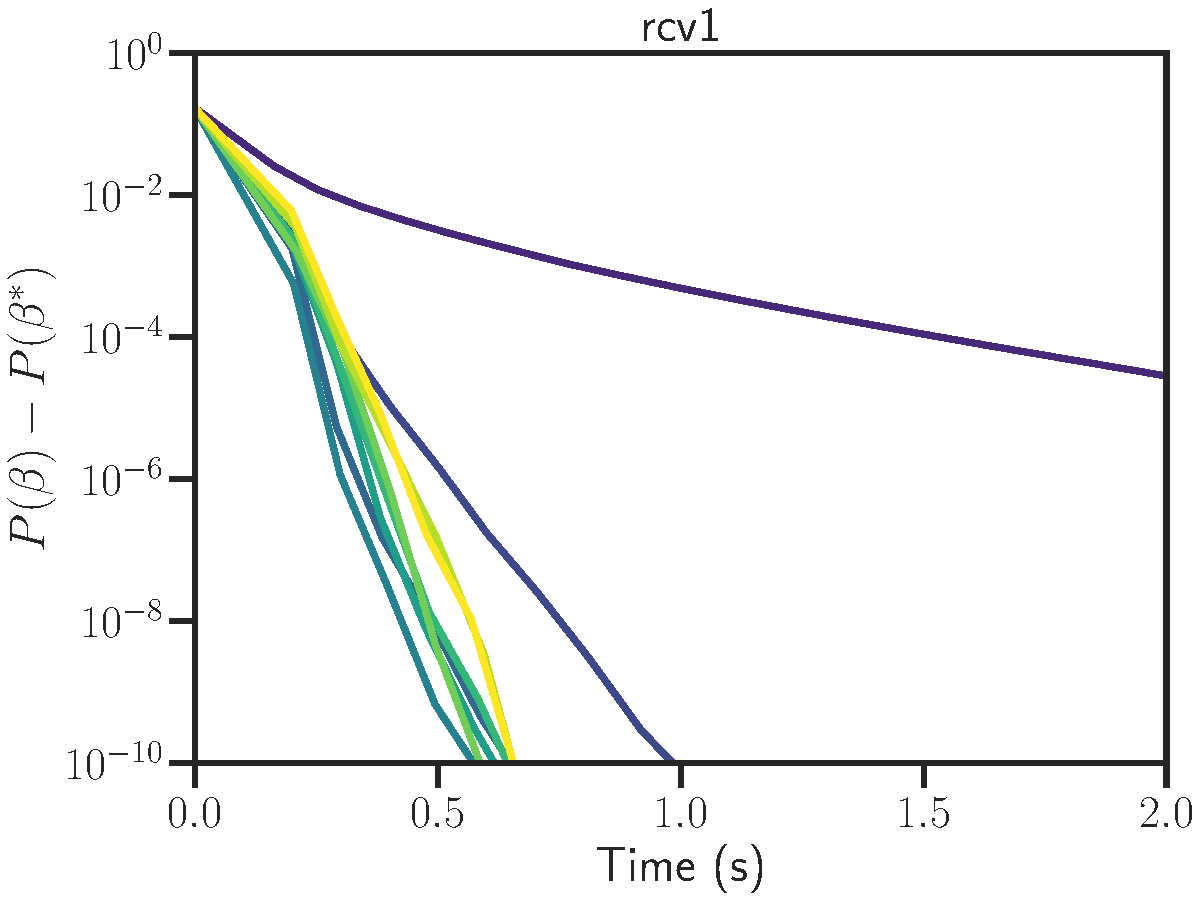
\includegraphics{pgd_freq.pdf}%
    \raisebox{0.585\height}{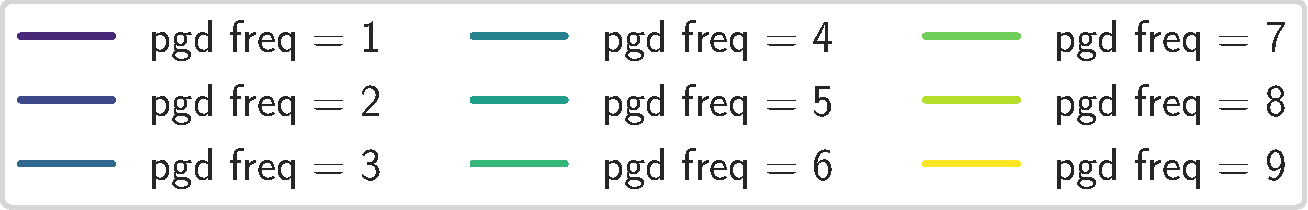
\includegraphics{pgd_freq_legend.pdf}}
    \caption{Suboptimality score as a function of the time for different frequencies of the PDG step inside the \texttt{hybrid} solver for the \dataset{rcv1} dataset}
  \label{fig:pgd_freq}
\end{figure*}

\subsection{Benchmark with Different Parameters for the ADMM Solver}
\label{sec:admm-benchmarks}

We reproduced the benchmarks setting described in \Cref{sec:experiments} for the simulated and real data.
We compared the \texttt{ADMM} solver with our \texttt{hybrid} algorithm for different values of the augmented Lagrangian parameter $\rho$.
We tested three different values $10, 100$ and $1000$ as well as the adaptive method~\parencite[Sec. 3.4.1]{boyd2010}.

We present in \Cref{fig:simulated_appendix} and \Cref{fig:real_appendix} the suboptimality score as a function the time for the different solvers.
We see that the best value for $\rho$ depends on the dataset and the regularization strengh.
The value chosen for the main benchmark (\Cref{sec:experiments}) performs well in comparison to other \texttt{ADMM} solvers.
Nevertheless, our \texttt{hybrid} approach is consistently faster than the different  \texttt{ADMM} solvers.

\begin{figure*}[!t]
  \centering
  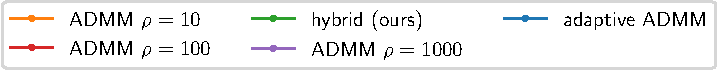
\includegraphics{simulated_legend_appendix.pdf}
  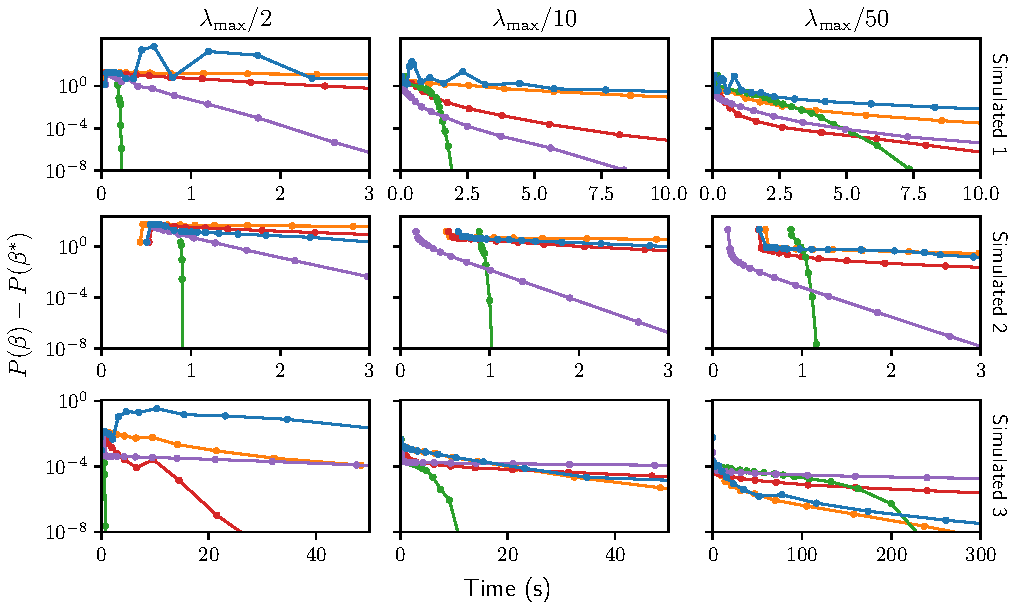
\includegraphics{simulated_appendix.pdf}
  \caption{\textbf{Benchmark on simulated datasets.} Suboptimality score as a function of time for SLOPE on multiple simulated datasets and for multiple sequence of $\lambda$.}
  \label{fig:simulated_appendix}
\end{figure*}


\begin{figure*}[!t]
  \centering
  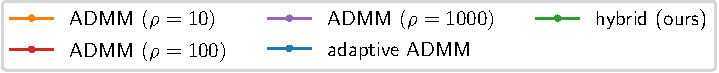
\includegraphics{real_legend_appendix.pdf}
  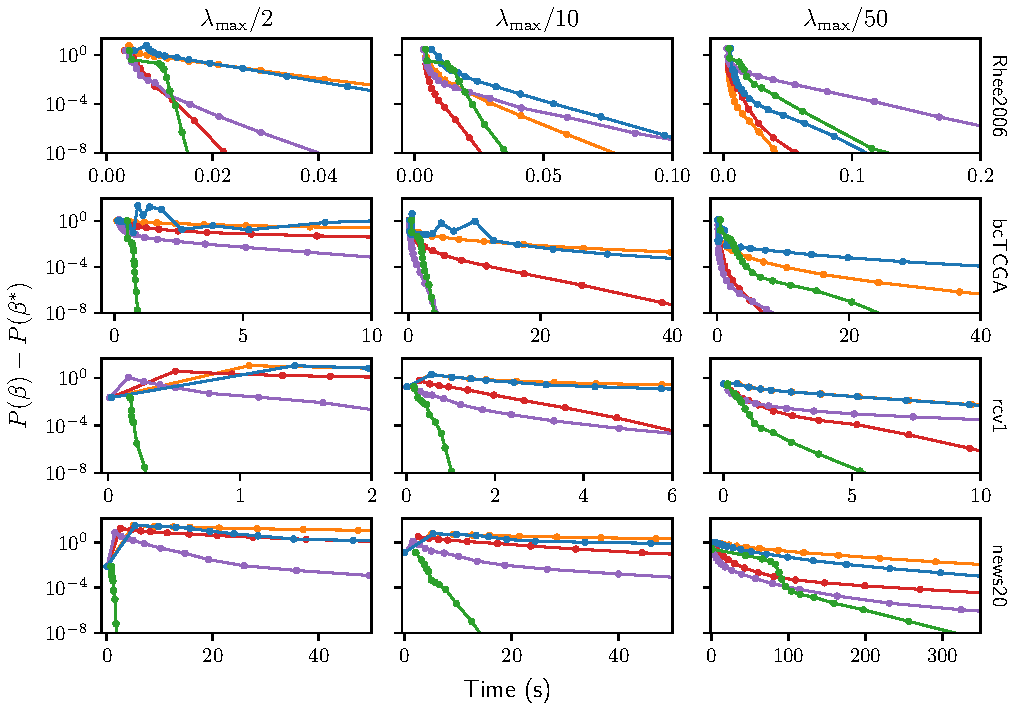
\includegraphics{real_appendix.pdf}
  \caption{\textbf{Benchmark on simulated datasets.} Suboptimality score as a function of time for SLOPE on multiple simulated datasets and for multiple sequence of $\lambda$.}
  \label{fig:real_appendix}
\end{figure*}

\subsection{SLOPE Path Benchmarks}
\label{sec:slope-path-benchmarks}

The choice of \(\lambda\) sequence in SLOPE is usually made via cross-validation on a training partition of the data across a grid of the \(q\) parameter, which controls the shape of the \(\lambda\) sequence, and \(\alpha\), a factor that scales the \(\lambda\) sequence.
The \(\alpha\) grid is typically a decreasing sequence where the first and last values correspond to the intercept-only and almost-saturated models respectively.
The set of models generated from fitting SLOPE across this grid of \(\alpha\) values is called the \emph{SLOPE path}. 
In this section, we report benchmarks on the performance of our algorithm in the case of fitting a SLOPE path to the simulated and real data sets used in \Cref{sec:experiments}.

We use the same path setup that is used by default for the lasso in the \pkg{glmnet} package~\parencite{friedman2010}. 
This entails using a grid of 100 \(\alpha\) values spaced evenly on the \(\log_e\)-scale.
The first value, \(\alpha_1\), is chosen such that it leads to the intercept-only model, that is \(\alpha_1\lambda = \lambda_\text{max}\)~(see \Cref{sec:experiments}).
The last value, \(\alpha_{100}\) is set to \(10^{-4}\) if \(p > n\) and \(10^{-2}\) otherwise.
We terminate the path early if the number of unique nonzero coefficients exceed \(n\)\footnote{Here we deviate from the standard lasso path setup because the lasso can at most select \(n\) nonzero coefficients, whilst SLOPE can select at most \(n\) nonzero \emph{unique} coefficients}, if the increase in the coefficient of determination is less than \(10^{-4}\) between two subsequent \(\alpha\)s on the path, or if the coefficient of determination equals or exceeds \(0.999\). 
The \(\lambda\) sequence setup, preprocessing, and data simulation setup is exactly the same as in \Cref{sec:experiments}.

For ADMM, we used \(\rho = 100\) following the results in \Cref{sec:admm-benchmarks}.
The Newt-ALM solver is missing from these benchmarks because we encountered several issues with convergence.

Our method outperforms the other methods for all of the real datasets~(\Cref{tab:path-real}).
In the case of \dataset{bcTCGA}, the difference is particularly striking, with our method taking less than one twentieth of the time taken for the runner-up. In the other cases, our method is roughly twice as fast as the second-best method.

\begin{table}[hbtp]
  \caption{Time in seconds to fit a full SLOPE path to real data sets. See \Cref{tab:real-data} for information about the datasets. For ADMM we set \(\rho = 100\).\label{tab:path-real}}
  \addtolength{\tabcolsep}{-2pt}
  \csvreader[
    tabular={
        l
        S[table-format=3.1]
        S[table-format=5.0]
        S[table-format=6.0]
        S[table-format=4.0]
      },
    before reading=\centering\sisetup{round-mode=places,round-precision=0},
    table head=\toprule Dataset & {\dataset{Rhee2006}} & {\dataset{bcTCGA}} & {\dataset{news20}} & {\dataset{rcv1}} \\\midrule,
    table foot=\bottomrule
  ]%
  {data/path_real.csv}%
  {Method=\method, Rhee2006=\rhee, bcTCGA=\bctcga, news20=\news, rcv1=\rcv}%
  {\method & \rhee & \bctcga & \news & \rcv}
\end{table}

For simulated data~(\Cref{tab:path-simulated}), our method performs best for the \(p > n\) scenarios (1 and 2), being roughly ten and five times faster, respectively, than the runner up.
In the case of Scenario 2 where \(n > p\), however, Anderson~(PGD) instead comes out on top. 

\begin{table}[hbtp]
  \caption{Time in seconds to fit a full SLOPE path to simulated data sets. See \Cref{tab:simulated-data} for information on what the different scenarios mean. For ADMM we set \(\rho = 100\).\label{tab:path-simulated}}
  \addtolength{\tabcolsep}{-2pt}
  \csvreader[
    tabular={
        l
        S[table-format=3.0]
        S[table-format=3.0]
        S[table-format=3.0]
      },
    before reading=\centering\sisetup{round-mode=places,round-precision=0},
    table head=\toprule Method & {Scenario 1} & {Scenario 2} & {Scenario 3} \\\midrule,
    table foot=\bottomrule
  ]%
  {data/path_simulated.csv}%
  {Method=\method, 1=\scea, 2=\sceb, 3=\scec}%
  {\method & \scea & \sceb & \scec}
\end{table}

This experiment was run on a dedicated high-performance computing cluster, using two Intel Xeon E5-2650 v3 (2.3 Ghz, 10-core) CPUs and 64~GB of memory.
The computations were enabled by resources provided by LUNARC.
